\normaltrue \difficilefalse \tdifficilefalse
\correctiontrue

%\UPSTIidClasse{11} % 11 sup, 12 spé
%\newcommand{\UPSTIidClasse}{12}

\exer{Pompe oscillante $\star$ \label{C2:06:13}}
\setcounter{question}{0}\UPSTIcompetence[2]{C2-06}
\index{Compétence C2-06}
\index{Pompe oscillante}

\ifcorrection
\else
\marginnote{\textbf{Pas de corrigé pour cet exercice.}}
\fi

\ifprof
\else

Soit le mécanisme suivant. On a $\vect{AB}=R\vect{i_1}$ et $\vect{CA}=H\vect{j_0}$. De plus, 
$R=\SI{40}{mm}$ et $H=\SI{60}{mm}$. Par ailleurs, on note $\vect{CB}=\lambda(t) \vect{i_2}$.


\begin{center}
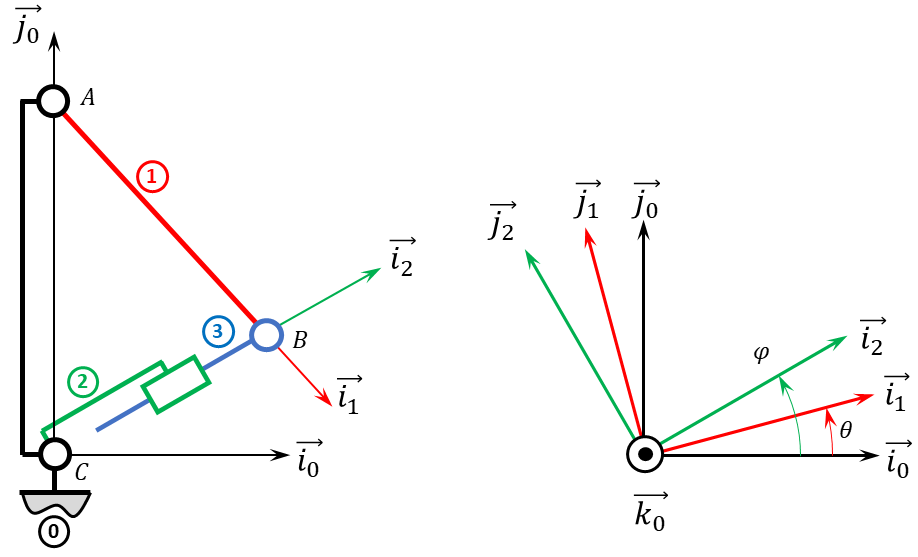
\includegraphics[width=\linewidth]{13_01}
\end{center}
\fi


\question{Tracer le graphe des liaisons.}

\ifprof

\begin{center}
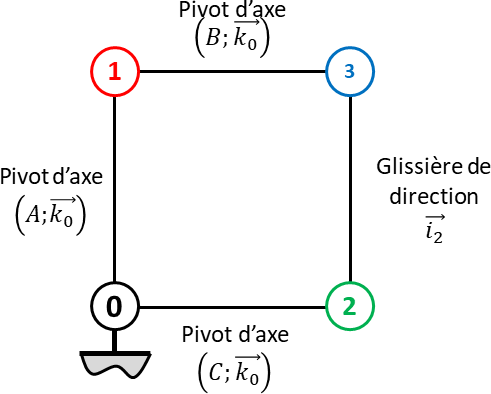
\includegraphics[width=.4\linewidth]{13_01_c}
\end{center}

\else
\fi

\question{Exprimer $\lambda(t)$ en fonction de $\theta(t)$.}

\ifprof

En réalisant une fermeture géométrique, on a $\vAB + \vBC + \vCA = \vect{0}$ 
$\Leftrightarrow R\vi{1} - \lambda(t)\vi{2} + H \vj{0}= \vect{0}$. 

En projetant cette expression dans le repère 
$\rep{0}$, on a 
$ R\left(\cos\theta(t) \vi{0}+\sin\theta(t) \vj{0} \right) - \lambda(t)\left(\cos\varphi(t) \vi{0}+\sin\varphi(t) \vj{0} \right) + H \vj{0} = \vect{0}$.

On obtient alors les équation scalaires suivantes : 
$\left\{
\begin{array}{l}
R\cos\theta(t) - \lambda(t)\cos\varphi(t)  = {0} \\
R\sin\theta(t)  - \lambda(t)\sin\varphi(t) + H  = {0} 
\end{array}
\right.
$.

On cherche à supprimer $\varphi(t)$, on va donc isoler la variable :
$\left\{
\begin{array}{l}
\lambda(t)\cos\varphi(t) = R\cos\theta(t)   \\
\lambda(t)\sin\varphi(t)  = R\sin\theta(t)  +H  
\end{array}
\right.
$.
$
\Rightarrow
\left\{
\begin{array}{l}
\lambda(t)^2\cos^2\varphi(t) = R^2\cos^2\theta(t)   \\
\lambda(t)^2\sin^2\varphi(t)  = \left(R\sin\theta(t)  +H \right)^2
\end{array}
\right.
$.
En sommant les expressions, on a : 
$\lambda(t)^2 =  R^2\cos^2\theta(t)  + \left(R\sin\theta(t)  +H \right)^2$.

Au final, 
$\lambda(t)^2 =  R^2  +H^2 +2 HR\sin\theta(t)$ et 

$\lambda(t) = \pm\sqrt{ R^2  +H^2 +2 HR\sin\theta(t)}$.
\else
\fi

\question{Exprimer $\dot{\lambda}(t)$ en fonction de $\dot{\theta}(t)$.}

\ifprof

En dérivant l'expression obtenue à la question précédente, on obtient 

$\lambdap(t) = \dfrac{1}{2}\left(-  2 HR\thetap(t)\cos\theta(t)\right)\left(R^2  +H^2 +2 HR\sin\theta(t)\right)^{-\dfrac{1}{2}}$.


\else
\fi


\question{Exprimer le débit instantané de la pompe. }

\ifprof
On note $q$ le débit instantané de la pompe. 
On a $q(t)=S\lambdap(t)$ avec $S$ la section du piston 3. 

\else
\fi

\question{En utilisant Python, donner le débit instantané de la pompe pour un tour de pompe pour un piston de diamètre $D=\SI{10}{mm}$.}

\ifprof

\begin{minipage}[c]{.3\linewidth}
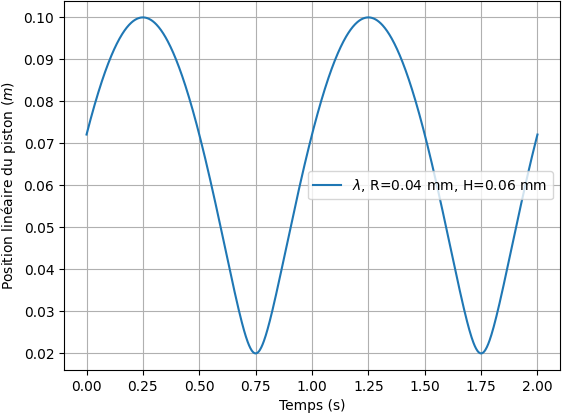
\includegraphics[width=\linewidth]{13_02_c}
\end{minipage}
\hfill
\begin{minipage}[c]{.3\linewidth}
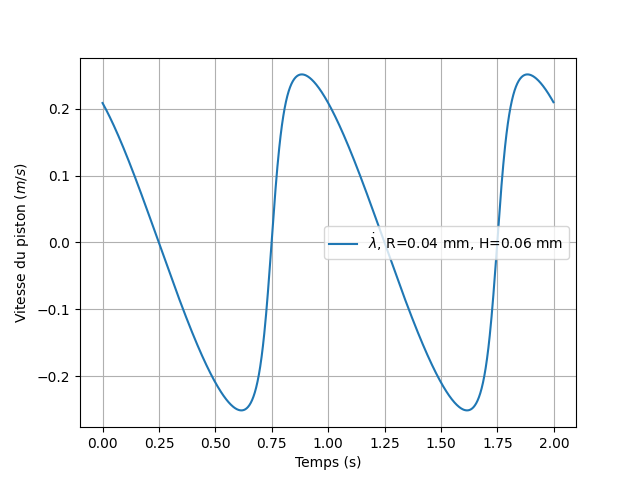
\includegraphics[width=\linewidth]{13_03_c}
\end{minipage}
\hfill
\begin{minipage}[c]{.3\linewidth}
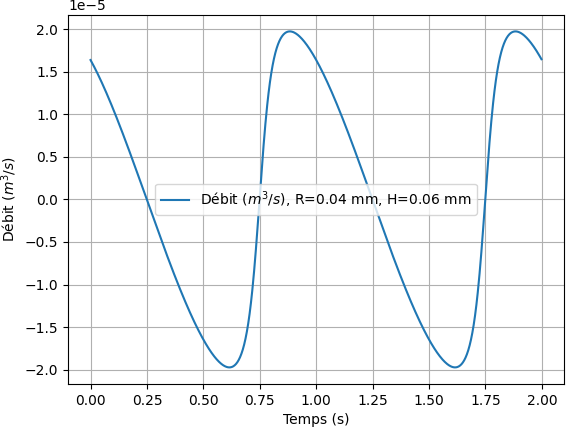
\includegraphics[width=\linewidth]{13_04_c}
\end{minipage}



\noindent\hrule
\begin{lstlisting}
#!/usr/bin/env python
# -*- coding: utf-8 -*-

"""13_TransfoMouvement.py"""

__author__ = "Xavier Pessoles"
__email__ = "xpessoles@lamartin.fr"

import numpy as np
import matplotlib.pyplot as plt
import math as m

R = 0.04 # m
H = 0.06     # m
D = 10e-3 # 10 mm

w = 60 # tours /min
w = w*2*m.pi/60  # rad/s

def calc_lambda(theta):
    res = R*R+H*H+2*H*R*np.sin(theta)
    
    return np.sqrt(res)

def calc_lambdap(theta):
    res = -H*R*w*np.cos(theta)*np.power(R*R+H*H+2*H*R*np.sin(theta),-0.5)
    return np.sqrt(res)

def calc_lambdap_bis(les_t,les_lambda):
    les_lambda_p = []
    for i in range(len(les_t)-1):
        les_lambda_p.append((les_lambda[i+1]-les_lambda[i])/(les_t[i+1]-les_t[i]))
        
    return les_lambda_p

def plot_lambda():
    les_t = np.linspace(0,2,1000)
    les_theta = w*les_t
    les_lambda = calc_lambda(les_theta)
    plt.grid()
    plt.xlabel("Temps (s)")
    plt.ylabel("Position linéaire du piston ($m$)")
    plt.plot(les_t,les_lambda,label=str("$\\lambda$, R=")+str(R)+" mm, "+str("H=")+str(H)+" mm")
    plt.legend()
    plt.show()

def plot_lambdap():
    les_t = np.linspace(0,2,1000)
    les_theta = w*les_t
    les_lambda = calc_lambda(les_theta)
    les_lambdap = calc_lambdap(les_theta)
    plt.grid()
    plt.xlabel("Temps (s)")
    plt.ylabel("Vitesse du piston ($m/s$)")
    #plt.plot(les_t,les_lambdap,label=str("$\dot{\\lambda}$, R=")+str(R)+" mm, "+str("H=")+str(H)+" mm")
    
    les_lambdap_bis = calc_lambdap_bis(les_t,les_lambda)
    plt.plot(les_t[:-1],les_lambdap_bis,label=str("$\dot{\\lambda}$, R=")+str(R)+" mm, "+str("H=")+str(H)+" mm")

    plt.legend()
    plt.show()
    
def plot_debit():
    les_t = np.linspace(0,2,1000)
    les_theta = w*les_t
    les_lambda = calc_lambda(les_theta)
    les_lambdap = calc_lambdap(les_theta)
    plt.grid()
    plt.xlabel("Temps (s)")
    plt.ylabel("Débit ($m^3/s$)")
    #plt.plot(les_t,les_lambdap,label=str("$\dot{\\lambda}$, R=")+str(R)+" mm, "+str("H=")+str(H)+" mm")
    
    les_lambdap_bis = calc_lambdap_bis(les_t,les_lambda)
    for i in range(len(les_lambdap_bis)):
        les_lambdap_bis[i]=les_lambdap_bis[i]*np.pi*D*D/4

    plt.plot(les_t[:-1],les_lambdap_bis,label=str("Débit ($m^3/s$), R=")+str(R)+" mm, "+str("H=")+str(H)+" mm")

    plt.legend()
    plt.show()
    
#plot_lambda()
#plot_lambdap()
plot_debit()


\end{lstlisting}
\noindent\hrule

\else
\fi




\ifprof
\else
\footnotesize
\ifcolle
\else
\begin{center}
\begin{tabular}{|p{.9\linewidth}|}
\hline
Indications :
\begin{enumerate}
\item .
\item $\lambda(t) = \pm\sqrt{ R^2  +H^2 +2 HR\sin\theta(t)}$
\item $\lambdap(t) = \dfrac{1}{2}\left(-  2 HR\thetap(t)\cos\theta(t)\right)\left(R^2  +H^2 +2 HR\sin\theta(t)\right)^{-\dfrac{1}{2}}$
\item $q(t)=S\lambdap(t)$
\item .
\end{enumerate} \\ \hline
\end{tabular}
\end{center}
\fi
\normalsize
\begin{flushright}
\footnotesize{Corrigé  voir \ref{C2:06:13}.}
\end{flushright}%
\fi